% ----------------------------------------------------------
% Introdução 
% Capítulo sem numeração, mas presente no Sumário
% ----------------------------------------------------------

\chapter[Introdução]{Introdução}
\addcontentsline{toc}{chapter}{Introdução}

A modernização dos processos faz com que seja necessário cada vez mais investimento em tecnologias de transmissão de informações e dados. Dispositivos como Controladores Lógicos Programáveis, placas microcontroladas como arduino e microcomputadores como o Raspberry são largamente aplicados e podem se utilizar das redes industriais para comunicação com dispositivos. O desenvolvimento das tecnologias de controle e comunicação possibilita para indústria a automatização cada vez mais efetivas de processos.

A atividade de desenvolver um supervisório que interligue o software Elipse E3 com o arduino consiste em uma aplicação prática de uma malha de comunicação, análogo ao que é encontrado normalmente na indústria. O arduino é um dispositivo que está se popularizando cada vez mais, não sendo a melhor solução em quesitos de preço e velocidade, mas se mostra prático e didático, assim conseguindo ilustrar os conhecimentos discutidos no decorrer da disciplina.



\section{Proposta}\label{sec:motivacao}
Desenvolver aplicação no software Elipse E3, que se comunica com a placa microcontrolada Arduino, utilizando os protocolos de comunicação MODBUS RTU e MODBUS TCP.

\subsection{Requisitos do Projeto}
\begin{itemize}
\item Apresentar uma interface gráfica no Sotfware Elipse E3 para comunicação com o usuário e display de informações
\item Receber um valor de um número decimal, converter para binário e mostrar no sistema de LEDS e na interface;
\item Apresentar status de botão conectado ao Arduino;
\item Fazer leitura do valor de um potênciometro, adicionar um \textit{offset} fornecido pelo usuário e apresentar na interface;
\end{itemize}
\section{Fundamentação teórica}
Para realização do trabalho foram necessários os seguintes conhecimentos relativos à redes e comunicações.
\subsection{Comunicação Serial}
Comunicação serial é a nomenclatura atribuída ao processo da troca de dados de forma sequencial por meio de um canal ou barramento específico para comunicação . Tais dados são bytes de informação, transmitidos bit a bit, por meio de uma porta serial.	

Os protocolos de comunicação serial representam o modo que a mensagem é transmitida, definindo a forma como os bytes serão ordenados de modo a garantir que a mensagem seja transmitida.
O padrão de comunicação diz respeito à estrutura física da comunicação, fazendo referência aos padrões elétricos envolvidos e quantidade de vias utilizadas.
\subsection{Protocolo MODBUS}
O protocolo MODBUS O protocolo Modbus é uma estrutura de mensagem aberta desenvolvida pela Modicon na década de 70. De acordo com a MODBUS Organization o protocolo MODBUS É:  “É um protocolo de camada de aplicação posicionado no nível 7 do modelo OSI , que fornece comunicação cliente / servidor entre dispositivos conectados em diferentes tipos de barramentos ou redes”. 

Consiste em um protocolo de solicitação/resposta , fornecendo serviços especificados por códigos de função. Os códigos de função de MODBUS são elementos das PDUs(Protocol Data Unit ou unidade de dados de protocolo) de solicitação / resposta de MODBUS.
É largamente utilizado em automação industrial, sendo transmitido por protocolos físicos como o RS232/RS485 e Ethernet TCP/IP. 

\subsubsection{Modo de transmissão RTU}
RTU é a sigla para Remote Terminal Unit, nesse modo de transmissão cada mensagem de dados de 8 bits contém dois caracteres hexadecimais de 4 bits, isso faz com que o processamento de dados seja mais rápido se comparado com a transmissão por 2 caracteres Ascii de 4 bits, já que a densidade de caracteres é maior. Apresenta 8 bits disponíveis para o endereço, 8 para função, 0 a 252 bits de data e 16 bits para o CRC Check, como mostrado na figura \ref{fig:rtu_packet} a seguir:
\begin{figure}[h]
	\centering
	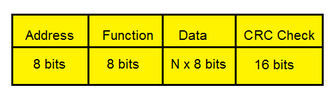
\includegraphics[width=.5\textwidth]{rtu_packet.png}
	\caption{Pacote da comunicação RTU}
	\label{fig:rtu_packet}
	%\source{Fornecido junto com os pontos}
\end{figure} 
\subsubsection{Modo de transmissão TCP}
O modo de transmissão TCP é uma aplicação do protocolo MODBUS baseado em TCP/IP, consequentemente utilizando a conexão ethernet. Para a pilha de comunicação, nesse protocolo é adicionado ao quadro um cabeçalho MBAP (MODBUS Application Protocol), deitando o modelo de mensagem como a figura \ref{fig:tcp_packet}:

\begin{figure}[h]
	\centering
	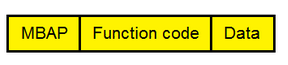
\includegraphics[width=.6\textwidth]{tcp_packet.png}
	\caption{Pacote da comunicação TCP}
	\label{fig:tcp_packet}
	%\source{Fornecido junto com os pontos}
\end{figure}
Esse novo cabeçalho tem 7 bytes de tamanho sendo composto por os seguintes elementos:
\begin{itemize}
	\item Transaction identifier: usado para identificação da resposta para a transação (2 bytes);
	\item Protocol identifier: 0 (zero) indica Modbus (2 bytes);
	\item Length: contagem de todos os próximos bytes (2 bytes);
	\item Unit identifier: utilizado para identificar o escravo remoto em uma rede Modbus RTU (1 byte).
	
\end{itemize}

O Modbus  TCP nao utiliza um byte de checkagem ao final da mensagem, pois o pŕoprio frame ethernet já apresenta uma checagem do tipo CRC-32. Na comunicação o cliente Modbus TCP inicia a conexão com o servidor para enviar as requisições, onde a porta padrão para a conexão com os servidores é a TCP 502.
